\documentclass[1p]{elsarticle_modified}
%\bibliographystyle{elsarticle-num}

%\usepackage[colorlinks]{hyperref}
%\usepackage{abbrmath_seonhwa} %\Abb, \Ascr, \Acal ,\Abf, \Afrak
\usepackage{amsfonts}
\usepackage{amssymb}
\usepackage{amsmath}
\usepackage{amsthm}
\usepackage{scalefnt}
\usepackage{amsbsy}
\usepackage{kotex}
\usepackage{caption}
\usepackage{subfig}
\usepackage{color}
\usepackage{graphicx}
\usepackage{xcolor} %% white, black, red, green, blue, cyan, magenta, yellow
\usepackage{float}
\usepackage{setspace}
\usepackage{hyperref}

\usepackage{tikz}
\usetikzlibrary{arrows}

\usepackage{multirow}
\usepackage{array} % fixed length table
\usepackage{hhline}

%%%%%%%%%%%%%%%%%%%%%
\makeatletter
\renewcommand*\env@matrix[1][\arraystretch]{%
	\edef\arraystretch{#1}%
	\hskip -\arraycolsep
	\let\@ifnextchar\new@ifnextchar
	\array{*\c@MaxMatrixCols c}}
\makeatother %https://tex.stackexchange.com/questions/14071/how-can-i-increase-the-line-spacing-in-a-matrix
%%%%%%%%%%%%%%%

\usepackage[normalem]{ulem}

\newcommand{\msout}[1]{\ifmmode\text{\sout{\ensuremath{#1}}}\else\sout{#1}\fi}
%SOURCE: \msout is \stkout macro in https://tex.stackexchange.com/questions/20609/strikeout-in-math-mode

\newcommand{\cancel}[1]{
	\ifmmode
	{\color{red}\msout{#1}}
	\else
	{\color{red}\sout{#1}}
	\fi
}

\newcommand{\add}[1]{
	{\color{blue}\uwave{#1}}
}

\newcommand{\replace}[2]{
	\ifmmode
	{\color{red}\msout{#1}}{\color{blue}\uwave{#2}}
	\else
	{\color{red}\sout{#1}}{\color{blue}\uwave{#2}}
	\fi
}

\newcommand{\Sol}{\mathcal{S}} %segment
\newcommand{\D}{D} %diagram
\newcommand{\A}{\mathcal{A}} %arc


%%%%%%%%%%%%%%%%%%%%%%%%%%%%%5 test

\def\sl{\operatorname{\textup{SL}}(2,\Cbb)}
\def\psl{\operatorname{\textup{PSL}}(2,\Cbb)}
\def\quan{\mkern 1mu \triangleright \mkern 1mu}

\theoremstyle{definition}
\newtheorem{thm}{Theorem}[section]
\newtheorem{prop}[thm]{Proposition}
\newtheorem{lem}[thm]{Lemma}
\newtheorem{ques}[thm]{Question}
\newtheorem{cor}[thm]{Corollary}
\newtheorem{defn}[thm]{Definition}
\newtheorem{exam}[thm]{Example}
\newtheorem{rmk}[thm]{Remark}
\newtheorem{alg}[thm]{Algorithm}

\newcommand{\I}{\sqrt{-1}}
\begin{document}

%\begin{frontmatter}
%
%\title{Boundary parabolic representations of knots up to 8 crossings}
%
%%% Group authors per affiliation:
%\author{Yunhi Cho} 
%\address{Department of Mathematics, University of Seoul, Seoul, Korea}
%\ead{yhcho@uos.ac.kr}
%
%
%\author{Seonhwa Kim} %\fnref{s_kim}}
%\address{Center for Geometry and Physics, Institute for Basic Science, Pohang, 37673, Korea}
%\ead{ryeona17@ibs.re.kr}
%
%\author{Hyuk Kim}
%\address{Department of Mathematical Sciences, Seoul National University, Seoul 08826, Korea}
%\ead{hyukkim@snu.ac.kr}
%
%\author{Seokbeom Yoon}
%\address{Department of Mathematical Sciences, Seoul National University, Seoul, 08826,  Korea}
%\ead{sbyoon15@snu.ac.kr}
%
%\begin{abstract}
%We find all boundary parabolic representation of knots up to 8 crossings.
%
%\end{abstract}
%\begin{keyword}
%    \MSC[2010] 57M25 
%\end{keyword}
%
%\end{frontmatter}

%\linenumbers
%\tableofcontents
%
\newcommand\colored[1]{\textcolor{white}{\rule[-0.35ex]{0.8em}{1.4ex}}\kern-0.8em\color{red} #1}%
%\newcommand\colored[1]{\textcolor{white}{ #1}\kern-2.17ex	\textcolor{white}{ #1}\kern-1.81ex	\textcolor{white}{ #1}\kern-2.15ex\color{red}#1	}

{\Large $\underline{12n_{0639}~(K12n_{0639})}$}

\setlength{\tabcolsep}{10pt}
\renewcommand{\arraystretch}{1.6}
\vspace{1cm}\begin{tabular}{m{100pt}>{\centering\arraybackslash}m{274pt}}
\multirow{5}{120pt}{
	\centering
	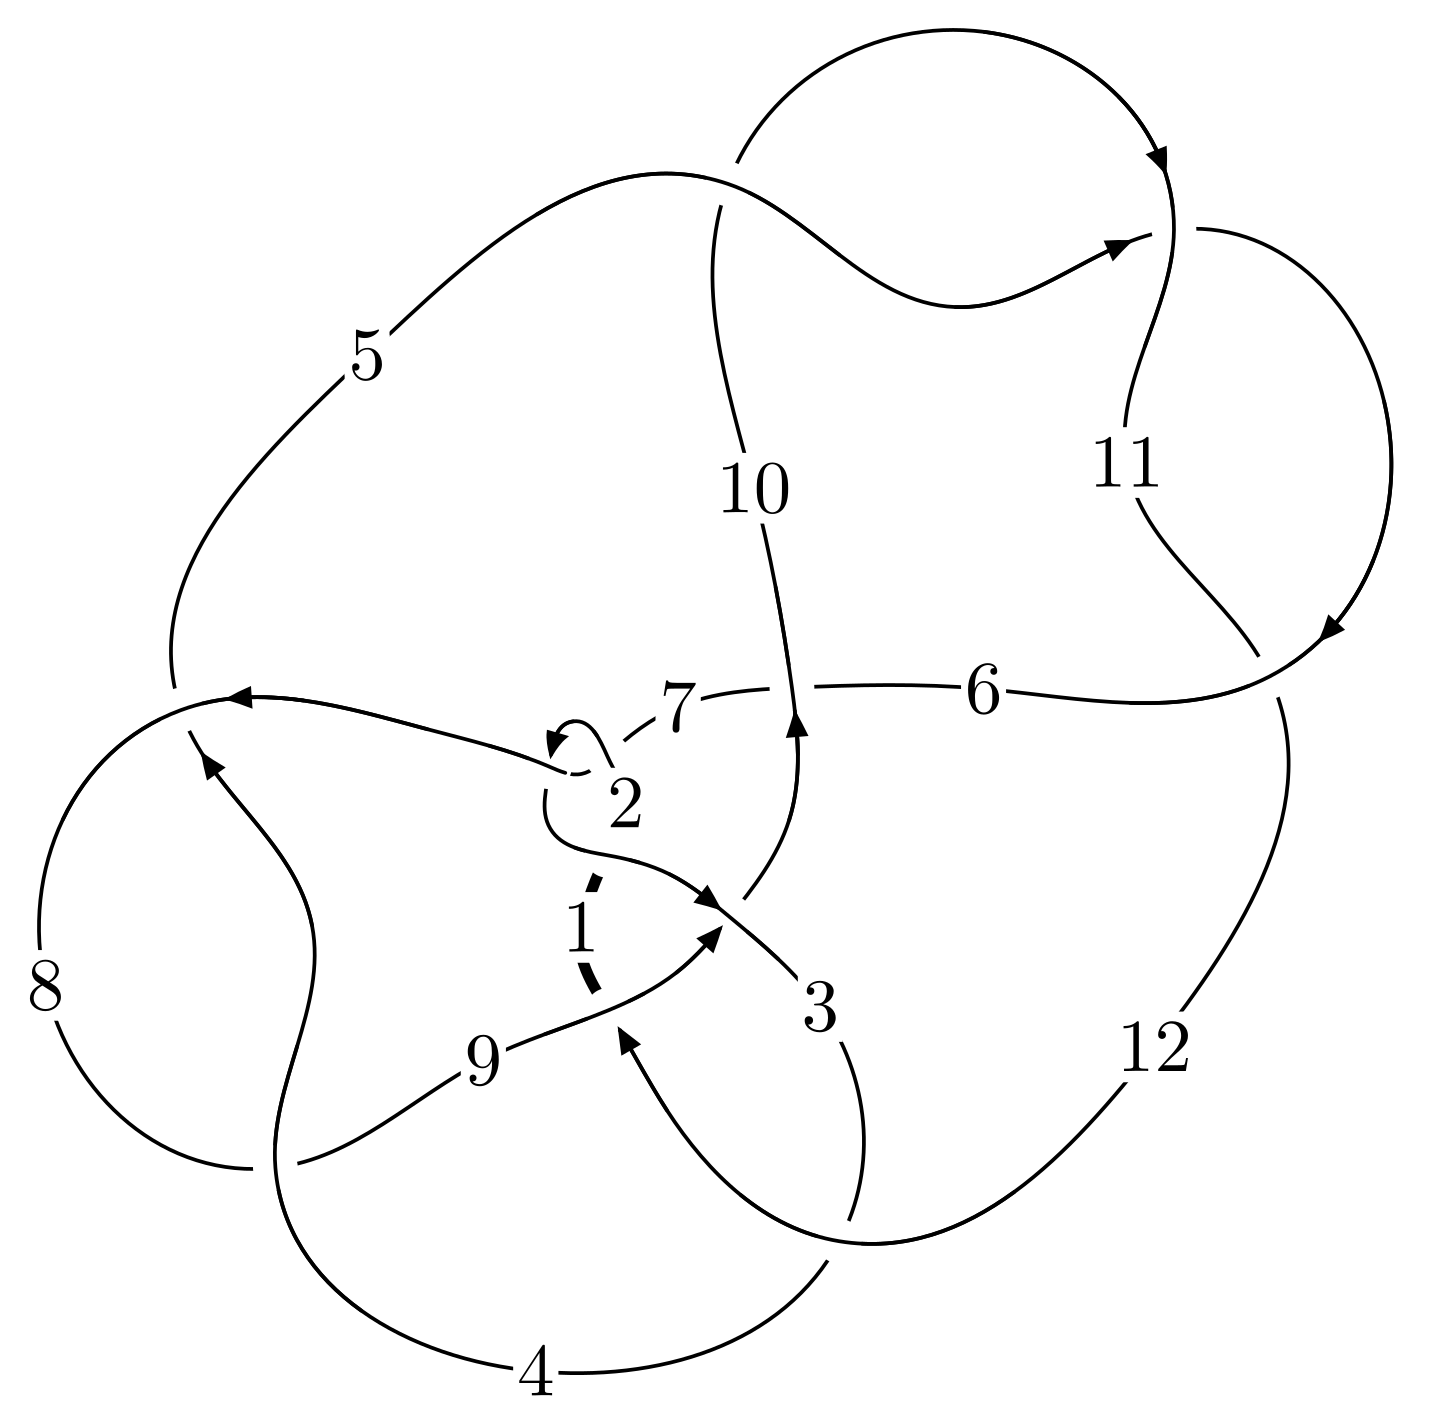
\includegraphics[width=112pt]{../../../GIT/diagram.site/Diagrams/png/2728_12n_0639.png}\\
\ \ \ A knot diagram\footnotemark}&
\allowdisplaybreaks
\textbf{Linearized knot diagam} \\
\cline{2-2}
 &
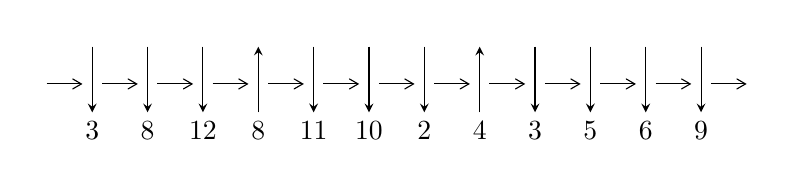
\begin{tikzpicture}[x=20pt, y=17pt]
	% nodes
	\node (C0) at (0, 0) {};
	\node (C1) at (1, 0) {};
	\node (C1U) at (1, +1) {};
	\node (C1D) at (1, -1) {3};

	\node (C2) at (2, 0) {};
	\node (C2U) at (2, +1) {};
	\node (C2D) at (2, -1) {8};

	\node (C3) at (3, 0) {};
	\node (C3U) at (3, +1) {};
	\node (C3D) at (3, -1) {12};

	\node (C4) at (4, 0) {};
	\node (C4U) at (4, +1) {};
	\node (C4D) at (4, -1) {8};

	\node (C5) at (5, 0) {};
	\node (C5U) at (5, +1) {};
	\node (C5D) at (5, -1) {11};

	\node (C6) at (6, 0) {};
	\node (C6U) at (6, +1) {};
	\node (C6D) at (6, -1) {10};

	\node (C7) at (7, 0) {};
	\node (C7U) at (7, +1) {};
	\node (C7D) at (7, -1) {2};

	\node (C8) at (8, 0) {};
	\node (C8U) at (8, +1) {};
	\node (C8D) at (8, -1) {4};

	\node (C9) at (9, 0) {};
	\node (C9U) at (9, +1) {};
	\node (C9D) at (9, -1) {3};

	\node (C10) at (10, 0) {};
	\node (C10U) at (10, +1) {};
	\node (C10D) at (10, -1) {5};

	\node (C11) at (11, 0) {};
	\node (C11U) at (11, +1) {};
	\node (C11D) at (11, -1) {6};

	\node (C12) at (12, 0) {};
	\node (C12U) at (12, +1) {};
	\node (C12D) at (12, -1) {9};
	\node (C13) at (13, 0) {};

	% arrows
	\draw[->,>={angle 60}]
	(C0) edge (C1) (C1) edge (C2) (C2) edge (C3) (C3) edge (C4) (C4) edge (C5) (C5) edge (C6) (C6) edge (C7) (C7) edge (C8) (C8) edge (C9) (C9) edge (C10) (C10) edge (C11) (C11) edge (C12) (C12) edge (C13) ;	\draw[->,>=stealth]
	(C1U) edge (C1D) (C2U) edge (C2D) (C3U) edge (C3D) (C4D) edge (C4U) (C5U) edge (C5D) (C6U) edge (C6D) (C7U) edge (C7D) (C8D) edge (C8U) (C9U) edge (C9D) (C10U) edge (C10D) (C11U) edge (C11D) (C12U) edge (C12D) ;
	\end{tikzpicture} \\
\hhline{~~} \\& 
\textbf{Solving Sequence} \\ \cline{2-2} 
 &
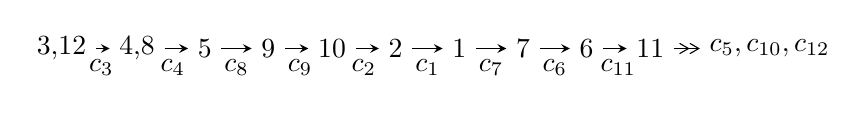
\begin{tikzpicture}[x=23pt, y=7pt]
	% node
	\node (A0) at (-1/8, 0) {3,12};
	\node (A1) at (17/16, 0) {4,8};
	\node (A2) at (17/8, 0) {5};
	\node (A3) at (25/8, 0) {9};
	\node (A4) at (33/8, 0) {10};
	\node (A5) at (41/8, 0) {2};
	\node (A6) at (49/8, 0) {1};
	\node (A7) at (57/8, 0) {7};
	\node (A8) at (65/8, 0) {6};
	\node (A9) at (73/8, 0) {11};
	\node (C1) at (1/2, -1) {$c_{3}$};
	\node (C2) at (13/8, -1) {$c_{4}$};
	\node (C3) at (21/8, -1) {$c_{8}$};
	\node (C4) at (29/8, -1) {$c_{9}$};
	\node (C5) at (37/8, -1) {$c_{2}$};
	\node (C6) at (45/8, -1) {$c_{1}$};
	\node (C7) at (53/8, -1) {$c_{7}$};
	\node (C8) at (61/8, -1) {$c_{6}$};
	\node (C9) at (69/8, -1) {$c_{11}$};
	\node (A10) at (11, 0) {$c_{5},c_{10},c_{12}$};

	% edge
	\draw[->,>=stealth]	
	(A0) edge (A1) (A1) edge (A2) (A2) edge (A3) (A3) edge (A4) (A4) edge (A5) (A5) edge (A6) (A6) edge (A7) (A7) edge (A8) (A8) edge (A9) ;
	\draw[->>,>={angle 60}]	
	(A9) edge (A10);
\end{tikzpicture} \\ 

\end{tabular} \\

\footnotetext{
The image of knot diagram is generated by the software ``\textbf{Draw programme}" developed by Andrew Bartholomew(\url{http://www.layer8.co.uk/maths/draw/index.htm\#Running-draw}), where we modified some parts for our purpose(\url{https://github.com/CATsTAILs/LinksPainter}).
}\phantom \\ \newline 
\centering \textbf{Ideals for irreducible components\footnotemark of $X_{\text{par}}$} 
 
\begin{align*}
I^u_{1}&=\langle 
11 u^{19}-95 u^{18}+\cdots+2 b-86,\;-49 u^{19}+435 u^{18}+\cdots+4 a+508,\;u^{20}-9 u^{19}+\cdots-22 u+4\rangle \\
I^u_{2}&=\langle 
u^{14}+4 u^{13}+10 u^{12}+15 u^{11}+15 u^{10}+6 u^9-6 u^8-16 u^7-16 u^6-13 u^5-6 u^4-3 u^3+b+u+2,\\
\phantom{I^u_{2}}&\phantom{= \langle  }-4 u^{14}-18 u^{13}+\cdots+a+5,\\
\phantom{I^u_{2}}&\phantom{= \langle  }u^{15}+6 u^{14}+19 u^{13}+38 u^{12}+50 u^{11}+37 u^{10}-4 u^9-52 u^8-74 u^7-57 u^6-18 u^5+12 u^4+18 u^3+8 u^2-1\rangle \\
I^u_{3}&=\langle 
- a^3-2 a^2 u+3 u^2 a- a^2+4 a u+u^2+b+3 a+u+3,\\
\phantom{I^u_{3}}&\phantom{= \langle  }a^3 u^2+a^4+2 a^3 u-5 a^2 u^2+a^3-4 a^2 u-3 u^2 a- a^2-5 a u-2 u^2-4 a-1,\;u^3+u^2-1\rangle \\
\\
\end{align*}
\raggedright * 3 irreducible components of $\dim_{\mathbb{C}}=0$, with total 47 representations.\\
\footnotetext{All coefficients of polynomials are rational numbers. But the coefficients are sometimes approximated in decimal forms when there is not enough margin.}
\newpage
\renewcommand{\arraystretch}{1}
\centering \section*{I. $I^u_{1}= \langle 11 u^{19}-95 u^{18}+\cdots+2 b-86,\;-49 u^{19}+435 u^{18}+\cdots+4 a+508,\;u^{20}-9 u^{19}+\cdots-22 u+4 \rangle$}
\flushleft \textbf{(i) Arc colorings}\\
\begin{tabular}{m{7pt} m{180pt} m{7pt} m{180pt} }
\flushright $a_{3}=$&$\begin{pmatrix}1\\0\end{pmatrix}$ \\
\flushright $a_{12}=$&$\begin{pmatrix}0\\u\end{pmatrix}$ \\
\flushright $a_{4}=$&$\begin{pmatrix}1\\u^2\end{pmatrix}$ \\
\flushright $a_{8}=$&$\begin{pmatrix}\frac{49}{4} u^{19}-\frac{435}{4} u^{18}+\cdots+\frac{1743}{4} u-127\\-\frac{11}{2} u^{19}+\frac{95}{2} u^{18}+\cdots-\frac{317}{2} u+43\end{pmatrix}$ \\
\flushright $a_{5}=$&$\begin{pmatrix}-\frac{1}{2} u^{19}+4 u^{18}+\cdots-\frac{27}{2} u+\frac{7}{2}\\-\frac{1}{2} u^{19}+\frac{7}{2} u^{18}+\cdots+6 u^2-\frac{1}{2} u\end{pmatrix}$ \\
\flushright $a_{9}=$&$\begin{pmatrix}\frac{43}{4} u^{19}-\frac{365}{4} u^{18}+\cdots+\frac{1173}{4} u-78\\\frac{1}{2} u^{19}-\frac{3}{2} u^{18}+\cdots-\frac{129}{2} u+27\end{pmatrix}$ \\
\flushright $a_{10}=$&$\begin{pmatrix}\frac{41}{4} u^{19}-\frac{359}{4} u^{18}+\cdots+\frac{1431}{4} u-105\\\frac{1}{2} u^{19}-\frac{3}{2} u^{18}+\cdots-\frac{129}{2} u+27\end{pmatrix}$ \\
\flushright $a_{2}=$&$\begin{pmatrix}\frac{1}{2} u^{18}-\frac{7}{2} u^{17}+\cdots-5 u+\frac{3}{2}\\\frac{1}{2} u^{19}-\frac{9}{2} u^{18}+\cdots+\frac{21}{2} u-2\end{pmatrix}$ \\
\flushright $a_{1}=$&$\begin{pmatrix}\frac{1}{2} u^{19}-4 u^{18}+\cdots+\frac{11}{2} u-\frac{1}{2}\\\frac{1}{2} u^{19}-\frac{9}{2} u^{18}+\cdots+\frac{21}{2} u-2\end{pmatrix}$ \\
\flushright $a_{7}=$&$\begin{pmatrix}12 u^{19}-\frac{209}{2} u^{18}+\cdots+404 u-\frac{237}{2}\\-\frac{13}{2} u^{19}+\frac{107}{2} u^{18}+\cdots-\frac{345}{2} u+48\end{pmatrix}$ \\
\flushright $a_{6}=$&$\begin{pmatrix}\frac{169}{4} u^{19}-\frac{1407}{4} u^{18}+\cdots+\frac{4055}{4} u-251\\-\frac{63}{2} u^{19}+\frac{521}{2} u^{18}+\cdots-\frac{1441}{2} u+173\end{pmatrix}$ \\
\flushright $a_{11}=$&$\begin{pmatrix}-\frac{55}{2} u^{19}+227 u^{18}+\cdots-\frac{1215}{2} u+\frac{285}{2}\\\frac{57}{2} u^{19}-\frac{469}{2} u^{18}+\cdots+\frac{1243}{2} u-146\end{pmatrix}$\\&\end{tabular}
\flushleft \textbf{(ii) Obstruction class $= -1$}\\~\\
\flushleft \textbf{(iii) Cusp Shapes $= 90 u^{19}-751 u^{18}+3199 u^{17}-8714 u^{16}+17011 u^{15}-25494 u^{14}+31435 u^{13}-32365 u^{12}+24669 u^{11}-4672 u^{10}-23026 u^9+47119 u^8-58278 u^7+55306 u^6-40524 u^5+20676 u^4-5078 u^3-2030 u^2+2210 u-566$}\\~\\
\newpage\renewcommand{\arraystretch}{1}
\flushleft \textbf{(iv) u-Polynomials at the component}\newline \\
\begin{tabular}{m{50pt}|m{274pt}}
Crossings & \hspace{64pt}u-Polynomials at each crossing \\
\hline $$\begin{aligned}c_{1}\end{aligned}$$&$\begin{aligned}
&u^{20}+35 u^{19}+\cdots-6 u+1
\end{aligned}$\\
\hline $$\begin{aligned}c_{2},c_{7},c_{12}\end{aligned}$$&$\begin{aligned}
&u^{20}+u^{19}+\cdots-2 u-1
\end{aligned}$\\
\hline $$\begin{aligned}c_{3}\end{aligned}$$&$\begin{aligned}
&u^{20}-9 u^{19}+\cdots-22 u+4
\end{aligned}$\\
\hline $$\begin{aligned}c_{4},c_{8}\end{aligned}$$&$\begin{aligned}
&u^{20}+15 u^{18}+\cdots-3 u-1
\end{aligned}$\\
\hline $$\begin{aligned}c_{5},c_{10},c_{11}\end{aligned}$$&$\begin{aligned}
&u^{20}-7 u^{19}+\cdots-16 u-8
\end{aligned}$\\
\hline $$\begin{aligned}c_{6}\end{aligned}$$&$\begin{aligned}
&u^{20}+21 u^{19}+\cdots+23824 u+2664
\end{aligned}$\\
\hline $$\begin{aligned}c_{9}\end{aligned}$$&$\begin{aligned}
&u^{20}-24 u^{18}+\cdots-197 u-57
\end{aligned}$\\
\hline
\end{tabular}\\~\\
\newpage\renewcommand{\arraystretch}{1}
\flushleft \textbf{(v) Riley Polynomials at the component}\newline \\
\begin{tabular}{m{50pt}|m{274pt}}
Crossings & \hspace{64pt}Riley Polynomials at each crossing \\
\hline $$\begin{aligned}c_{1}\end{aligned}$$&$\begin{aligned}
&y^{20}-123 y^{19}+\cdots-118 y+1
\end{aligned}$\\
\hline $$\begin{aligned}c_{2},c_{7},c_{12}\end{aligned}$$&$\begin{aligned}
&y^{20}-35 y^{19}+\cdots+6 y+1
\end{aligned}$\\
\hline $$\begin{aligned}c_{3}\end{aligned}$$&$\begin{aligned}
&y^{20}+y^{19}+\cdots-172 y+16
\end{aligned}$\\
\hline $$\begin{aligned}c_{4},c_{8}\end{aligned}$$&$\begin{aligned}
&y^{20}+30 y^{19}+\cdots-41 y+1
\end{aligned}$\\
\hline $$\begin{aligned}c_{5},c_{10},c_{11}\end{aligned}$$&$\begin{aligned}
&y^{20}-19 y^{19}+\cdots-352 y+64
\end{aligned}$\\
\hline $$\begin{aligned}c_{6}\end{aligned}$$&$\begin{aligned}
&y^{20}-7 y^{19}+\cdots-72537184 y+7096896
\end{aligned}$\\
\hline $$\begin{aligned}c_{9}\end{aligned}$$&$\begin{aligned}
&y^{20}-48 y^{19}+\cdots+66527 y+3249
\end{aligned}$\\
\hline
\end{tabular}\\~\\
\newpage\flushleft \textbf{(vi) Complex Volumes and Cusp Shapes}
$$\begin{array}{c|c|c}  
\text{Solutions to }I^u_{1}& \I (\text{vol} + \sqrt{-1}CS) & \text{Cusp shape}\\
 \hline 
\begin{aligned}
u &= -0.263775 + 0.933613 I \\
a &= \phantom{-}0.063867 + 0.469394 I \\
b &= \phantom{-}0.635043 - 0.343749 I\end{aligned}
 & \phantom{-}1.90324 + 1.62770 I & -2.35623 - 4.39456 I \\ \hline\begin{aligned}
u &= -0.263775 - 0.933613 I \\
a &= \phantom{-}0.063867 - 0.469394 I \\
b &= \phantom{-}0.635043 + 0.343749 I\end{aligned}
 & \phantom{-}1.90324 - 1.62770 I & -2.35623 + 4.39456 I \\ \hline\begin{aligned}
u &= -1.08046\phantom{ +0.000000I} \\
a &= \phantom{-}0.288950\phantom{ +0.000000I} \\
b &= \phantom{-}0.649514\phantom{ +0.000000I}\end{aligned}
 & -5.71917\phantom{ +0.000000I} & -17.5810\phantom{ +0.000000I} \\ \hline\begin{aligned}
u &= \phantom{-}0.288783 + 0.801332 I \\
a &= \phantom{-}0.234474 - 0.843337 I \\
b &= -0.484200 + 0.635373 I\end{aligned}
 & -2.01141 - 1.38113 I & -7.57284 - 0.08377 I \\ \hline\begin{aligned}
u &= \phantom{-}0.288783 - 0.801332 I \\
a &= \phantom{-}0.234474 + 0.843337 I \\
b &= -0.484200 - 0.635373 I\end{aligned}
 & -2.01141 + 1.38113 I & -7.57284 + 0.08377 I \\ \hline\begin{aligned}
u &= -0.626429 + 1.085280 I \\
a &= -0.082861 - 0.296469 I \\
b &= -0.711687 + 0.249730 I\end{aligned}
 & -2.18377 + 5.21287 I & -7.17987 - 5.41855 I \\ \hline\begin{aligned}
u &= -0.626429 - 1.085280 I \\
a &= -0.082861 + 0.296469 I \\
b &= -0.711687 - 0.249730 I\end{aligned}
 & -2.18377 - 5.21287 I & -7.17987 + 5.41855 I \\ \hline\begin{aligned}
u &= \phantom{-}0.727091 + 0.098566 I \\
a &= \phantom{-}0.27452 - 2.08093 I \\
b &= \phantom{-}0.036016 + 0.445425 I\end{aligned}
 & -6.93044 - 4.62901 I & -12.95845 - 0.90844 I \\ \hline\begin{aligned}
u &= \phantom{-}0.727091 - 0.098566 I \\
a &= \phantom{-}0.27452 + 2.08093 I \\
b &= \phantom{-}0.036016 - 0.445425 I\end{aligned}
 & -6.93044 + 4.62901 I & -12.95845 + 0.90844 I \\ \hline\begin{aligned}
u &= \phantom{-}0.622736 + 0.087717 I \\
a &= -0.13935 + 1.89543 I \\
b &= -0.007001 - 0.462890 I\end{aligned}
 & -1.13986 - 1.75347 I & -8.00254 + 2.62344 I\\
 \hline 
 \end{array}$$\newpage$$\begin{array}{c|c|c}  
\text{Solutions to }I^u_{1}& \I (\text{vol} + \sqrt{-1}CS) & \text{Cusp shape}\\
 \hline 
\begin{aligned}
u &= \phantom{-}0.622736 - 0.087717 I \\
a &= -0.13935 - 1.89543 I \\
b &= -0.007001 + 0.462890 I\end{aligned}
 & -1.13986 + 1.75347 I & -8.00254 - 2.62344 I \\ \hline\begin{aligned}
u &= \phantom{-}1.15558 + 1.02594 I \\
a &= \phantom{-}0.454735 + 1.318780 I \\
b &= -2.17085 - 0.53930 I\end{aligned}
 & \phantom{-}17.3877 - 12.0858 I & -13.7130 + 4.9422 I \\ \hline\begin{aligned}
u &= \phantom{-}1.15558 - 1.02594 I \\
a &= \phantom{-}0.454735 - 1.318780 I \\
b &= -2.17085 + 0.53930 I\end{aligned}
 & \phantom{-}17.3877 + 12.0858 I & -13.7130 - 4.9422 I \\ \hline\begin{aligned}
u &= \phantom{-}1.04701 + 1.18287 I \\
a &= -0.989116 - 0.564620 I \\
b &= \phantom{-}2.06593 - 0.51777 I\end{aligned}
 & \phantom{-}17.9143 + 3.9437 I & -13.79737 - 1.18244 I \\ \hline\begin{aligned}
u &= \phantom{-}1.04701 - 1.18287 I \\
a &= -0.989116 + 0.564620 I \\
b &= \phantom{-}2.06593 + 0.51777 I\end{aligned}
 & \phantom{-}17.9143 - 3.9437 I & -13.79737 + 1.18244 I \\ \hline\begin{aligned}
u &= -0.408607\phantom{ +0.000000I} \\
a &= -0.763027\phantom{ +0.000000I} \\
b &= -0.439173\phantom{ +0.000000I}\end{aligned}
 & -0.693185\phantom{ +0.000000I} & -14.4620\phantom{ +0.000000I} \\ \hline\begin{aligned}
u &= \phantom{-}1.16573 + 1.09145 I \\
a &= -0.587075 - 1.041030 I \\
b &= \phantom{-}2.09877 + 0.18587 I\end{aligned}
 & -14.6724 - 7.3263 I & -11.70204 + 4.29722 I \\ \hline\begin{aligned}
u &= \phantom{-}1.16573 - 1.09145 I \\
a &= -0.587075 + 1.041030 I \\
b &= \phantom{-}2.09877 - 0.18587 I\end{aligned}
 & -14.6724 + 7.3263 I & -11.70204 - 4.29722 I \\ \hline\begin{aligned}
u &= \phantom{-}1.12782 + 1.15737 I \\
a &= \phantom{-}0.757846 + 0.799117 I \\
b &= -2.06719 + 0.14611 I\end{aligned}
 & -14.4635 - 1.0817 I & -11.69610 + 0. I\phantom{ +0.000000I} \\ \hline\begin{aligned}
u &= \phantom{-}1.12782 - 1.15737 I \\
a &= \phantom{-}0.757846 - 0.799117 I \\
b &= -2.06719 - 0.14611 I\end{aligned}
 & -14.4635 + 1.0817 I & -11.69610 + 0. I\phantom{ +0.000000I}\\
 \hline 
 \end{array}$$\newpage\newpage\renewcommand{\arraystretch}{1}
\centering \section*{II. $I^u_{2}= \langle u^{14}+4 u^{13}+\cdots+b+2,\;-4 u^{14}-18 u^{13}+\cdots+a+5,\;u^{15}+6 u^{14}+\cdots+8 u^2-1 \rangle$}
\flushleft \textbf{(i) Arc colorings}\\
\begin{tabular}{m{7pt} m{180pt} m{7pt} m{180pt} }
\flushright $a_{3}=$&$\begin{pmatrix}1\\0\end{pmatrix}$ \\
\flushright $a_{12}=$&$\begin{pmatrix}0\\u\end{pmatrix}$ \\
\flushright $a_{4}=$&$\begin{pmatrix}1\\u^2\end{pmatrix}$ \\
\flushright $a_{8}=$&$\begin{pmatrix}4 u^{14}+18 u^{13}+\cdots-11 u-5\\- u^{14}-4 u^{13}+\cdots- u-2\end{pmatrix}$ \\
\flushright $a_{5}=$&$\begin{pmatrix}- u^{12}-5 u^{11}+\cdots-10 u-7\\- u^{14}-6 u^{13}+\cdots-17 u^2-8 u\end{pmatrix}$ \\
\flushright $a_{9}=$&$\begin{pmatrix}-2 u^{14}-13 u^{13}+\cdots-16 u-1\\-4 u^{14}-22 u^{13}+\cdots-7 u+3\end{pmatrix}$ \\
\flushright $a_{10}=$&$\begin{pmatrix}2 u^{14}+9 u^{13}+\cdots-9 u-4\\-4 u^{14}-22 u^{13}+\cdots-7 u+3\end{pmatrix}$ \\
\flushright $a_{2}=$&$\begin{pmatrix}- u^{13}-6 u^{12}+\cdots-18 u-7\\- u^{14}-6 u^{13}+\cdots-8 u-1\end{pmatrix}$ \\
\flushright $a_{1}=$&$\begin{pmatrix}- u^{14}-7 u^{13}+\cdots-26 u-8\\- u^{14}-6 u^{13}+\cdots-8 u-1\end{pmatrix}$ \\
\flushright $a_{7}=$&$\begin{pmatrix}4 u^{14}+22 u^{13}+\cdots+29 u+9\\2 u^{14}+13 u^{13}+\cdots+16 u+1\end{pmatrix}$ \\
\flushright $a_{6}=$&$\begin{pmatrix}-2 u^{14}-11 u^{13}+\cdots+4 u+7\\4 u^{14}+24 u^{13}+\cdots+12 u-6\end{pmatrix}$ \\
\flushright $a_{11}=$&$\begin{pmatrix}5 u^{14}+29 u^{13}+\cdots+22 u-2\\-4 u^{14}-23 u^{13}+\cdots-4 u+9\end{pmatrix}$\\&\end{tabular}
\flushleft \textbf{(ii) Obstruction class $= 1$}\\~\\
\flushleft \textbf{(iii) Cusp Shapes $= 15 u^{14}+84 u^{13}+246 u^{12}+446 u^{11}+504 u^{10}+245 u^9-262 u^8-701 u^7-742 u^6-398 u^5+24 u^4+221 u^3+159 u^2+17 u-32$}\\~\\
\newpage\renewcommand{\arraystretch}{1}
\flushleft \textbf{(iv) u-Polynomials at the component}\newline \\
\begin{tabular}{m{50pt}|m{274pt}}
Crossings & \hspace{64pt}u-Polynomials at each crossing \\
\hline $$\begin{aligned}c_{1}\end{aligned}$$&$\begin{aligned}
&u^{15}-15 u^{14}+\cdots+9 u-1
\end{aligned}$\\
\hline $$\begin{aligned}c_{2}\end{aligned}$$&$\begin{aligned}
&u^{15}+u^{14}+\cdots- u-1
\end{aligned}$\\
\hline $$\begin{aligned}c_{3}\end{aligned}$$&$\begin{aligned}
&u^{15}+6 u^{14}+\cdots+8 u^2-1
\end{aligned}$\\
\hline $$\begin{aligned}c_{4}\end{aligned}$$&$\begin{aligned}
&u^{15}+3 u^{13}+\cdots-4 u^2-1
\end{aligned}$\\
\hline $$\begin{aligned}c_{5}\end{aligned}$$&$\begin{aligned}
&u^{15}-8 u^{13}+\cdots-12 u^3-1
\end{aligned}$\\
\hline $$\begin{aligned}c_{6}\end{aligned}$$&$\begin{aligned}
&u^{15}+8 u^{12}+\cdots+3 u^2-1
\end{aligned}$\\
\hline $$\begin{aligned}c_{7},c_{12}\end{aligned}$$&$\begin{aligned}
&u^{15}- u^{14}+\cdots- u+1
\end{aligned}$\\
\hline $$\begin{aligned}c_{8}\end{aligned}$$&$\begin{aligned}
&u^{15}+3 u^{13}+\cdots+4 u^2+1
\end{aligned}$\\
\hline $$\begin{aligned}c_{9}\end{aligned}$$&$\begin{aligned}
&u^{15}-8 u^{13}+\cdots+2 u^2+1
\end{aligned}$\\
\hline $$\begin{aligned}c_{10},c_{11}\end{aligned}$$&$\begin{aligned}
&u^{15}-8 u^{13}+\cdots-12 u^3+1
\end{aligned}$\\
\hline
\end{tabular}\\~\\
\newpage\renewcommand{\arraystretch}{1}
\flushleft \textbf{(v) Riley Polynomials at the component}\newline \\
\begin{tabular}{m{50pt}|m{274pt}}
Crossings & \hspace{64pt}Riley Polynomials at each crossing \\
\hline $$\begin{aligned}c_{1}\end{aligned}$$&$\begin{aligned}
&y^{15}-31 y^{14}+\cdots-11 y-1
\end{aligned}$\\
\hline $$\begin{aligned}c_{2},c_{7},c_{12}\end{aligned}$$&$\begin{aligned}
&y^{15}-15 y^{14}+\cdots+9 y-1
\end{aligned}$\\
\hline $$\begin{aligned}c_{3}\end{aligned}$$&$\begin{aligned}
&y^{15}+2 y^{14}+\cdots+16 y-1
\end{aligned}$\\
\hline $$\begin{aligned}c_{4},c_{8}\end{aligned}$$&$\begin{aligned}
&y^{15}+6 y^{14}+\cdots-8 y-1
\end{aligned}$\\
\hline $$\begin{aligned}c_{5},c_{10},c_{11}\end{aligned}$$&$\begin{aligned}
&y^{15}-16 y^{14}+\cdots+12 y^2-1
\end{aligned}$\\
\hline $$\begin{aligned}c_{6}\end{aligned}$$&$\begin{aligned}
&y^{15}-22 y^{13}+\cdots+6 y-1
\end{aligned}$\\
\hline $$\begin{aligned}c_{9}\end{aligned}$$&$\begin{aligned}
&y^{15}-16 y^{14}+\cdots-4 y-1
\end{aligned}$\\
\hline
\end{tabular}\\~\\
\newpage\flushleft \textbf{(vi) Complex Volumes and Cusp Shapes}
$$\begin{array}{c|c|c}  
\text{Solutions to }I^u_{2}& \I (\text{vol} + \sqrt{-1}CS) & \text{Cusp shape}\\
 \hline 
\begin{aligned}
u &= \phantom{-}1.02838\phantom{ +0.000000I} \\
a &= -0.673279\phantom{ +0.000000I} \\
b &= -1.40442\phantom{ +0.000000I}\end{aligned}
 & -8.97607\phantom{ +0.000000I} & -19.1120\phantom{ +0.000000I} \\ \hline\begin{aligned}
u &= -0.865049 + 0.608135 I \\
a &= -0.280256 + 1.131020 I \\
b &= \phantom{-}0.638534 - 0.425883 I\end{aligned}
 & -1.66725 + 3.23030 I & -7.54630 - 5.89815 I \\ \hline\begin{aligned}
u &= -0.865049 - 0.608135 I \\
a &= -0.280256 - 1.131020 I \\
b &= \phantom{-}0.638534 + 0.425883 I\end{aligned}
 & -1.66725 - 3.23030 I & -7.54630 + 5.89815 I \\ \hline\begin{aligned}
u &= -0.034033 + 1.074520 I \\
a &= -0.708776 - 0.233805 I \\
b &= \phantom{-}1.075770 - 0.432119 I\end{aligned}
 & -3.77019 - 2.56256 I & -12.71337 + 2.06324 I \\ \hline\begin{aligned}
u &= -0.034033 - 1.074520 I \\
a &= -0.708776 + 0.233805 I \\
b &= \phantom{-}1.075770 + 0.432119 I\end{aligned}
 & -3.77019 + 2.56256 I & -12.71337 - 2.06324 I \\ \hline\begin{aligned}
u &= -0.764295 + 0.414957 I \\
a &= \phantom{-}0.38774 - 1.74222 I \\
b &= -0.518757 + 0.528802 I\end{aligned}
 & -6.94753 + 5.39923 I & -13.2804 - 8.9655 I \\ \hline\begin{aligned}
u &= -0.764295 - 0.414957 I \\
a &= \phantom{-}0.38774 + 1.74222 I \\
b &= -0.518757 - 0.528802 I\end{aligned}
 & -6.94753 - 5.39923 I & -13.2804 + 8.9655 I \\ \hline\begin{aligned}
u &= -0.410448 + 1.166870 I \\
a &= \phantom{-}0.612112 - 0.171673 I \\
b &= -0.945688 + 0.403215 I\end{aligned}
 & \phantom{-}0.60597 + 1.58539 I & -9.91315 - 2.10632 I \\ \hline\begin{aligned}
u &= -0.410448 - 1.166870 I \\
a &= \phantom{-}0.612112 + 0.171673 I \\
b &= -0.945688 - 0.403215 I\end{aligned}
 & \phantom{-}0.60597 - 1.58539 I & -9.91315 + 2.10632 I \\ \hline\begin{aligned}
u &= -1.122950 + 0.658583 I \\
a &= -0.067419 - 0.819750 I \\
b &= -0.652697 + 0.297689 I\end{aligned}
 & -5.15231 + 1.54512 I & -15.9184 - 2.4740 I\\
 \hline 
 \end{array}$$\newpage$$\begin{array}{c|c|c}  
\text{Solutions to }I^u_{2}& \I (\text{vol} + \sqrt{-1}CS) & \text{Cusp shape}\\
 \hline 
\begin{aligned}
u &= -1.122950 - 0.658583 I \\
a &= -0.067419 + 0.819750 I \\
b &= -0.652697 - 0.297689 I\end{aligned}
 & -5.15231 - 1.54512 I & -15.9184 + 2.4740 I \\ \hline\begin{aligned}
u &= \phantom{-}0.625489\phantom{ +0.000000I} \\
a &= \phantom{-}1.58555\phantom{ +0.000000I} \\
b &= \phantom{-}1.61206\phantom{ +0.000000I}\end{aligned}
 & -6.43860\phantom{ +0.000000I} & -4.48120\phantom{ +0.000000I} \\ \hline\begin{aligned}
u &= -0.76860 + 1.27462 I \\
a &= -0.362430 + 0.320539 I \\
b &= \phantom{-}0.872760 - 0.329613 I\end{aligned}
 & -2.95721 + 5.51163 I & -16.1590 - 8.3531 I \\ \hline\begin{aligned}
u &= -0.76860 - 1.27462 I \\
a &= -0.362430 - 0.320539 I \\
b &= \phantom{-}0.872760 + 0.329613 I\end{aligned}
 & -2.95721 - 5.51163 I & -16.1590 + 8.3531 I \\ \hline\begin{aligned}
u &= \phantom{-}0.276879\phantom{ +0.000000I} \\
a &= -6.07420\phantom{ +0.000000I} \\
b &= -2.14748\phantom{ +0.000000I}\end{aligned}
 & -13.8955\phantom{ +0.000000I} & -11.3460\phantom{ +0.000000I}\\
 \hline 
 \end{array}$$\newpage\newpage\renewcommand{\arraystretch}{1}
\centering \section*{III. $I^u_{3}= \langle 3 u^2 a+u^2+\cdots+3 a+3,\;a^3 u^2-5 a^2 u^2+\cdots-4 a-1,\;u^3+u^2-1 \rangle$}
\flushleft \textbf{(i) Arc colorings}\\
\begin{tabular}{m{7pt} m{180pt} m{7pt} m{180pt} }
\flushright $a_{3}=$&$\begin{pmatrix}1\\0\end{pmatrix}$ \\
\flushright $a_{12}=$&$\begin{pmatrix}0\\u\end{pmatrix}$ \\
\flushright $a_{4}=$&$\begin{pmatrix}1\\u^2\end{pmatrix}$ \\
\flushright $a_{8}=$&$\begin{pmatrix}a\\a^3+2 a^2 u-3 u^2 a+a^2-4 a u- u^2-3 a- u-3\end{pmatrix}$ \\
\flushright $a_{5}=$&$\begin{pmatrix}a^3 u^2- a^2 u^2-2 u^2 a+2 a^2-4 a u-2 u^2- a\\-2 a^3 u^2+3 a^2 u^2+4 u^2 a-4 a^2+8 a u+4 u^2+2 a-2 u\end{pmatrix}$ \\
\flushright $a_{9}=$&$\begin{pmatrix}a^3+2 a^2 u-4 u^2 a+a^2-4 a u- u^2-2 a- u-3\\a^3 u^2- a^2 u^2+a^3+2 a^2 u-6 u^2 a+3 a^2-8 a u-4 u^2-3 a-2 u-3\end{pmatrix}$ \\
\flushright $a_{10}=$&$\begin{pmatrix}- a^3 u^2+a^2 u^2+2 u^2 a-2 a^2+4 a u+3 u^2+a+u\\a^3 u^2- a^2 u^2+a^3+2 a^2 u-6 u^2 a+3 a^2-8 a u-4 u^2-3 a-2 u-3\end{pmatrix}$ \\
\flushright $a_{2}=$&$\begin{pmatrix}a^3 u^2-2 a^2 u^2-2 u^2 a+2 a^2-4 a u-2 u^2- a\\- a^3 u^2+a^3 u+3 a^2 u^2- a^3-2 a^2 u+5 u^2 a-2 a^2+6 a u-4 u+2\end{pmatrix}$ \\
\flushright $a_{1}=$&$\begin{pmatrix}a^3 u+a^2 u^2- a^3-2 a^2 u+3 u^2 a+2 a u-2 u^2- a-4 u+2\\- a^3 u^2+a^3 u+3 a^2 u^2- a^3-2 a^2 u+5 u^2 a-2 a^2+6 a u-4 u+2\end{pmatrix}$ \\
\flushright $a_{7}=$&$\begin{pmatrix}3 a^3 u^2-3 a^2 u^2-6 u^2 a+6 a^2-12 a u-8 u^2-3 a-2 u\\-5 a^3 u^2+4 a^2 u^2+\cdots+10 a+4\end{pmatrix}$ \\
\flushright $a_{6}=$&$\begin{pmatrix}a^3 u^2- a^2 u^2-2 u^2 a+2 a^2-4 a u-3 u^2- a- u\\-2 a^3 u^2- a^3 u- a^2 u+5 u^2 a-4 a^2+10 a u+6 u^2+5 a+5 u+1\end{pmatrix}$ \\
\flushright $a_{11}=$&$\begin{pmatrix}a^3 u^2- a^2 u^2-2 u^2 a+2 a^2-4 a u-2 u^2- a\\-3 a^3 u^2+2 a^2 u^2+\cdots+4 a-2\end{pmatrix}$\\&\end{tabular}
\flushleft \textbf{(ii) Obstruction class $= -1$}\\~\\
\flushleft \textbf{(iii) Cusp Shapes $= -4 u-18$}\\~\\
\newpage\renewcommand{\arraystretch}{1}
\flushleft \textbf{(iv) u-Polynomials at the component}\newline \\
\begin{tabular}{m{50pt}|m{274pt}}
Crossings & \hspace{64pt}u-Polynomials at each crossing \\
\hline $$\begin{aligned}c_{1}\end{aligned}$$&$\begin{aligned}
&u^{12}+21 u^{11}+\cdots+54160 u+10201
\end{aligned}$\\
\hline $$\begin{aligned}c_{2},c_{7},c_{12}\end{aligned}$$&$\begin{aligned}
&u^{12}- u^{11}+\cdots-78 u+101
\end{aligned}$\\
\hline $$\begin{aligned}c_{3}\end{aligned}$$&$\begin{aligned}
&(u^3+u^2-1)^4
\end{aligned}$\\
\hline $$\begin{aligned}c_{4},c_{8}\end{aligned}$$&$\begin{aligned}
&u^{12}-3 u^{11}+\cdots+110 u-19
\end{aligned}$\\
\hline $$\begin{aligned}c_{5},c_{10},c_{11}\end{aligned}$$&$\begin{aligned}
&(u^2+u-1)^6
\end{aligned}$\\
\hline $$\begin{aligned}c_{6}\end{aligned}$$&$\begin{aligned}
&(u^2-3 u+1)^6
\end{aligned}$\\
\hline $$\begin{aligned}c_{9}\end{aligned}$$&$\begin{aligned}
&u^{12}- u^{11}+\cdots+170 u+211
\end{aligned}$\\
\hline
\end{tabular}\\~\\
\newpage\renewcommand{\arraystretch}{1}
\flushleft \textbf{(v) Riley Polynomials at the component}\newline \\
\begin{tabular}{m{50pt}|m{274pt}}
Crossings & \hspace{64pt}Riley Polynomials at each crossing \\
\hline $$\begin{aligned}c_{1}\end{aligned}$$&$\begin{aligned}
&y^{12}-37 y^{11}+\cdots-490778160 y+104060401
\end{aligned}$\\
\hline $$\begin{aligned}c_{2},c_{7},c_{12}\end{aligned}$$&$\begin{aligned}
&y^{12}-21 y^{11}+\cdots-54160 y+10201
\end{aligned}$\\
\hline $$\begin{aligned}c_{3}\end{aligned}$$&$\begin{aligned}
&(y^3- y^2+2 y-1)^4
\end{aligned}$\\
\hline $$\begin{aligned}c_{4},c_{8}\end{aligned}$$&$\begin{aligned}
&y^{12}+7 y^{11}+\cdots-7160 y+361
\end{aligned}$\\
\hline $$\begin{aligned}c_{5},c_{10},c_{11}\end{aligned}$$&$\begin{aligned}
&(y^2-3 y+1)^6
\end{aligned}$\\
\hline $$\begin{aligned}c_{6}\end{aligned}$$&$\begin{aligned}
&(y^2-7 y+1)^6
\end{aligned}$\\
\hline $$\begin{aligned}c_{9}\end{aligned}$$&$\begin{aligned}
&y^{12}-29 y^{11}+\cdots-124272 y+44521
\end{aligned}$\\
\hline
\end{tabular}\\~\\
\newpage\flushleft \textbf{(vi) Complex Volumes and Cusp Shapes}
$$\begin{array}{c|c|c}  
\text{Solutions to }I^u_{3}& \I (\text{vol} + \sqrt{-1}CS) & \text{Cusp shape}\\
 \hline 
\begin{aligned}
u &= -0.877439 + 0.744862 I \\
a &= \phantom{-}0.290927 - 0.889122 I \\
b &= -0.901307 + 0.772844 I\end{aligned}
 & -2.89763 + 2.82812 I & -14.4902 - 2.9794 I \\ \hline\begin{aligned}
u &= -0.877439 + 0.744862 I \\
a &= -0.624540 + 1.001960 I \\
b &= \phantom{-}0.768380 + 0.035014 I\end{aligned}
 & -2.89763 + 2.82812 I & -14.4902 - 2.9794 I \\ \hline\begin{aligned}
u &= -0.877439 + 0.744862 I \\
a &= -0.550642 + 1.189890 I \\
b &= \phantom{-}1.58009 - 1.38831 I\end{aligned}
 & -10.79330 + 2.82812 I & -14.4902 - 2.9794 I \\ \hline\begin{aligned}
u &= -0.877439 + 0.744862 I \\
a &= \phantom{-}1.42405 - 1.48532 I \\
b &= -1.23208 - 0.72669 I\end{aligned}
 & -10.79330 + 2.82812 I & -14.4902 - 2.9794 I \\ \hline\begin{aligned}
u &= -0.877439 - 0.744862 I \\
a &= \phantom{-}0.290927 + 0.889122 I \\
b &= -0.901307 - 0.772844 I\end{aligned}
 & -2.89763 - 2.82812 I & -14.4902 + 2.9794 I \\ \hline\begin{aligned}
u &= -0.877439 - 0.744862 I \\
a &= -0.624540 - 1.001960 I \\
b &= \phantom{-}0.768380 - 0.035014 I\end{aligned}
 & -2.89763 - 2.82812 I & -14.4902 + 2.9794 I \\ \hline\begin{aligned}
u &= -0.877439 - 0.744862 I \\
a &= -0.550642 - 1.189890 I \\
b &= \phantom{-}1.58009 + 1.38831 I\end{aligned}
 & -10.79330 - 2.82812 I & -14.4902 + 2.9794 I \\ \hline\begin{aligned}
u &= -0.877439 - 0.744862 I \\
a &= \phantom{-}1.42405 + 1.48532 I \\
b &= -1.23208 + 0.72669 I\end{aligned}
 & -10.79330 - 2.82812 I & -14.4902 + 2.9794 I \\ \hline\begin{aligned}
u &= \phantom{-}0.754878\phantom{ +0.000000I} \\
a &= -0.777477\phantom{ +0.000000I} \\
b &= \phantom{-}2.73154\phantom{ +0.000000I}\end{aligned}
 & -14.9309\phantom{ +0.000000I} & -21.0200\phantom{ +0.000000I} \\ \hline\begin{aligned}
u &= \phantom{-}0.754878\phantom{ +0.000000I} \\
a &= -0.297371\phantom{ +0.000000I} \\
b &= -1.83069\phantom{ +0.000000I}\end{aligned}
 & -7.03522\phantom{ +0.000000I} & -21.0200\phantom{ +0.000000I}\\
 \hline 
 \end{array}$$\newpage$$\begin{array}{c|c|c}  
\text{Solutions to }I^u_{3}& \I (\text{vol} + \sqrt{-1}CS) & \text{Cusp shape}\\
 \hline 
\begin{aligned}
u &= \phantom{-}0.754878\phantom{ +0.000000I} \\
a &= \phantom{-}2.20067\phantom{ +0.000000I} \\
b &= \phantom{-}1.47851\phantom{ +0.000000I}\end{aligned}
 & -7.03522\phantom{ +0.000000I} & -21.0200\phantom{ +0.000000I} \\ \hline\begin{aligned}
u &= \phantom{-}0.754878\phantom{ +0.000000I} \\
a &= -4.20541\phantom{ +0.000000I} \\
b &= -1.80951\phantom{ +0.000000I}\end{aligned}
 & -14.9309\phantom{ +0.000000I} & -21.0200\phantom{ +0.000000I}\\
 \hline 
 \end{array}$$\newpage
\newpage\renewcommand{\arraystretch}{1}
\centering \section*{ IV. u-Polynomials}
\begin{tabular}{m{50pt}|m{274pt}}
Crossings & \hspace{64pt}u-Polynomials at each crossing \\
\hline $$\begin{aligned}c_{1}\end{aligned}$$&$\begin{aligned}
&(u^{12}+21 u^{11}+\cdots+54160 u+10201)(u^{15}-15 u^{14}+\cdots+9 u-1)\\
&\cdot(u^{20}+35 u^{19}+\cdots-6 u+1)
\end{aligned}$\\
\hline $$\begin{aligned}c_{2}\end{aligned}$$&$\begin{aligned}
&(u^{12}- u^{11}+\cdots-78 u+101)(u^{15}+u^{14}+\cdots- u-1)\\
&\cdot(u^{20}+u^{19}+\cdots-2 u-1)
\end{aligned}$\\
\hline $$\begin{aligned}c_{3}\end{aligned}$$&$\begin{aligned}
&((u^3+u^2-1)^4)(u^{15}+6 u^{14}+\cdots+8 u^2-1)(u^{20}-9 u^{19}+\cdots-22 u+4)
\end{aligned}$\\
\hline $$\begin{aligned}c_{4}\end{aligned}$$&$\begin{aligned}
&(u^{12}-3 u^{11}+\cdots+110 u-19)(u^{15}+3 u^{13}+\cdots-4 u^2-1)\\
&\cdot(u^{20}+15 u^{18}+\cdots-3 u-1)
\end{aligned}$\\
\hline $$\begin{aligned}c_{5}\end{aligned}$$&$\begin{aligned}
&((u^2+u-1)^6)(u^{15}-8 u^{13}+\cdots-12 u^3-1)(u^{20}-7 u^{19}+\cdots-16 u-8)
\end{aligned}$\\
\hline $$\begin{aligned}c_{6}\end{aligned}$$&$\begin{aligned}
&((u^2-3 u+1)^6)(u^{15}+8 u^{12}+\cdots+3 u^2-1)\\
&\cdot(u^{20}+21 u^{19}+\cdots+23824 u+2664)
\end{aligned}$\\
\hline $$\begin{aligned}c_{7},c_{12}\end{aligned}$$&$\begin{aligned}
&(u^{12}- u^{11}+\cdots-78 u+101)(u^{15}- u^{14}+\cdots- u+1)\\
&\cdot(u^{20}+u^{19}+\cdots-2 u-1)
\end{aligned}$\\
\hline $$\begin{aligned}c_{8}\end{aligned}$$&$\begin{aligned}
&(u^{12}-3 u^{11}+\cdots+110 u-19)(u^{15}+3 u^{13}+\cdots+4 u^2+1)\\
&\cdot(u^{20}+15 u^{18}+\cdots-3 u-1)
\end{aligned}$\\
\hline $$\begin{aligned}c_{9}\end{aligned}$$&$\begin{aligned}
&(u^{12}- u^{11}+\cdots+170 u+211)(u^{15}-8 u^{13}+\cdots+2 u^2+1)\\
&\cdot(u^{20}-24 u^{18}+\cdots-197 u-57)
\end{aligned}$\\
\hline $$\begin{aligned}c_{10},c_{11}\end{aligned}$$&$\begin{aligned}
&((u^2+u-1)^6)(u^{15}-8 u^{13}+\cdots-12 u^3+1)(u^{20}-7 u^{19}+\cdots-16 u-8)
\end{aligned}$\\
\hline
\end{tabular}\newpage\renewcommand{\arraystretch}{1}
\centering \section*{ V. Riley Polynomials}
\begin{tabular}{m{50pt}|m{274pt}}
Crossings & \hspace{64pt}Riley Polynomials at each crossing \\
\hline $$\begin{aligned}c_{1}\end{aligned}$$&$\begin{aligned}
&(y^{12}-37 y^{11}+\cdots-490778160 y+104060401)\\
&\cdot(y^{15}-31 y^{14}+\cdots-11 y-1)(y^{20}-123 y^{19}+\cdots-118 y+1)
\end{aligned}$\\
\hline $$\begin{aligned}c_{2},c_{7},c_{12}\end{aligned}$$&$\begin{aligned}
&(y^{12}-21 y^{11}+\cdots-54160 y+10201)(y^{15}-15 y^{14}+\cdots+9 y-1)\\
&\cdot(y^{20}-35 y^{19}+\cdots+6 y+1)
\end{aligned}$\\
\hline $$\begin{aligned}c_{3}\end{aligned}$$&$\begin{aligned}
&((y^3- y^2+2 y-1)^4)(y^{15}+2 y^{14}+\cdots+16 y-1)\\
&\cdot(y^{20}+y^{19}+\cdots-172 y+16)
\end{aligned}$\\
\hline $$\begin{aligned}c_{4},c_{8}\end{aligned}$$&$\begin{aligned}
&(y^{12}+7 y^{11}+\cdots-7160 y+361)(y^{15}+6 y^{14}+\cdots-8 y-1)\\
&\cdot(y^{20}+30 y^{19}+\cdots-41 y+1)
\end{aligned}$\\
\hline $$\begin{aligned}c_{5},c_{10},c_{11}\end{aligned}$$&$\begin{aligned}
&((y^2-3 y+1)^6)(y^{15}-16 y^{14}+\cdots+12 y^2-1)\\
&\cdot(y^{20}-19 y^{19}+\cdots-352 y+64)
\end{aligned}$\\
\hline $$\begin{aligned}c_{6}\end{aligned}$$&$\begin{aligned}
&((y^2-7 y+1)^6)(y^{15}-22 y^{13}+\cdots+6 y-1)\\
&\cdot(y^{20}-7 y^{19}+\cdots-72537184 y+7096896)
\end{aligned}$\\
\hline $$\begin{aligned}c_{9}\end{aligned}$$&$\begin{aligned}
&(y^{12}-29 y^{11}+\cdots-124272 y+44521)(y^{15}-16 y^{14}+\cdots-4 y-1)\\
&\cdot(y^{20}-48 y^{19}+\cdots+66527 y+3249)
\end{aligned}$\\
\hline
\end{tabular}
\vskip 2pc
\end{document}